\chapter{Continuous Integration e Continuous Deployment}

\section*{Introduzione}
Continuous Integration (CI) e Continuous Deployment (CD) sono pratiche fondamentali dello sviluppo moderno. CI automatizza testing e verifica del codice ad ogni commit. CD automatizza il deployment in produzione. Questo capitolo introduce i concetti e implementa pipeline CI/CD con GitHub Actions.

\section*{Obiettivi di apprendimento}
\begin{itemize}
    \item Comprendere concetti di CI/CD e benefici
    \item Configurare pipeline GitHub Actions
    \item Implementare testing automatico
    \item Automatizzare build e deployment
    \item Gestire secrets e environment variables
    \item Usare matrix builds per multi-platform testing
    \item Implementare deployment strategies
    \item Monitorare e debuggare pipeline
\end{itemize}

\section{Cos'è CI/CD}

\subsection{Continuous Integration (CI)}

\textbf{Definizione}: Pratica di integrare codice nel repository principale frequentemente (più volte al giorno), con verifica automatica tramite build e test.

Il workflow tradizionale senza CI presenta problemi significativi. Tipicamente, uno sviluppatore lavora sul codice per giorni o addirittura settimane in isolamento prima di fare commit e push. A quel punto inizia l'integrazione manuale con il codice scritto da altri membri del team, processo durante il quale emergono bug e conflitti che erano rimasti nascosti. I fix richiesti sono spesso lunghi e dolorosi perché il codice non è più fresco nella memoria dello sviluppatore e i problemi si sono accumulati.

Al contrario, il workflow con CI trasforma radicalmente questo processo. Lo sviluppatore continua a scrivere codice ma fa commit e push frequenti, múltiple volte al giorno. Ad ogni push, il server CI interviene automaticamente compilando il codice, eseguendo i test e verificando che tutto funzioni. Questo fornisce feedback immediato su eventuali errori, permettendo fix rapidi mentre il codice è ancora fresco nella memoria dello sviluppatore. I problemi vengono identificati e risolti quando sono piccoli, prima che si accumulino e diventino complessi.

\subsection{Continuous Deployment (CD)}

\textbf{Definizione}: Estensione di CI che automatizza deployment in produzione dopo successful build/test.

\textbf{Varianti}:
\begin{description}
    \item[Continuous Delivery] Codice sempre pronto per deploy, ma deploy manuale
    \item[Continuous Deployment] Deploy automatico in produzione ad ogni commit
\end{description}

\subsection{Benefici CI/CD}

\begin{tcolorbox}[colback=green!10, colframe=green!60, title=Vantaggi]
\begin{itemize}
    \item \textbf{Feedback rapido}: Scopri errori subito, non dopo giorni
    \item \textbf{Qualità codice}: Test automatici prevengono regressioni
    \item \textbf{Deployment veloce}: Da commit a produzione in minuti
    \item \textbf{Riduzione rischio}: Deploy piccoli e frequenti vs grandi release
    \item \textbf{Automazione}: Meno errori umani
    \item \textbf{Confidence}: Deploy sicuri grazie a test completi
\end{itemize}
\end{tcolorbox}

\section{Pipeline CI/CD: Concetti}

\subsection{Anatomia di una Pipeline}

\begin{center}
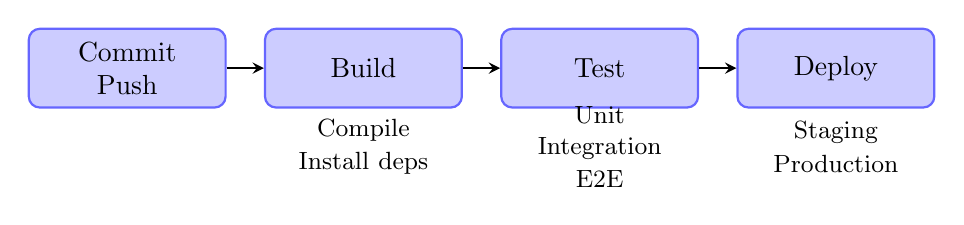
\begin{tikzpicture}[
    node distance=1.5cm,
    stage/.style={rectangle, rounded corners, draw=blue!60, fill=blue!20, thick, minimum width=2.5cm, minimum height=1cm, align=center},
    arrow/.style={->, thick, >=stealth}
]
    \node[stage] (commit) {Commit\\Push};
    \node[stage, right of=commit, xshift=1.5cm] (build) {Build};
    \node[stage, right of=build, xshift=1.5cm] (test) {Test};
    \node[stage, right of=test, xshift=1.5cm] (deploy) {Deploy};

    \draw[arrow] (commit) -- (build);
    \draw[arrow] (build) -- (test);
    \draw[arrow] (test) -- (deploy);

    \node[below of=build, yshift=0.5cm, text width=2cm, align=center] {\small Compile\\Install deps};
    \node[below of=test, yshift=0.5cm, text width=2cm, align=center] {\small Unit\\Integration\\E2E};
    \node[below of=deploy, yshift=0.5cm, text width=2cm, align=center] {\small Staging\\Production};
\end{tikzpicture}
\end{center}

\subsection{Pipeline Completa con Branch}

\begin{center}
\begin{tikzpicture}[
    node distance=0.8cm and 1.2cm,
    stage/.style={rectangle, rounded corners, draw=blue!60, fill=blue!20, thick, minimum width=2cm, minimum height=0.8cm, align=center, font=\small},
    success/.style={rectangle, rounded corners, draw=green!60, fill=green!20, thick, minimum width=2cm, minimum height=0.8cm, align=center, font=\small},
    fail/.style={rectangle, rounded corners, draw=red!60, fill=red!20, thick, minimum width=2cm, minimum height=0.8cm, align=center, font=\small},
    arrow/.style={->, thick, >=stealth},
    decision/.style={diamond, draw=orange!60, fill=orange!20, thick, minimum width=1cm, align=center, font=\small}
]
    % Feature branch flow
    \node[stage] (feature) {Feature\\Branch};
    \node[stage, right=of feature] (lint) {Lint\\Code};
    \node[stage, right=of lint] (unit) {Unit\\Tests};
    \node[decision, right=of unit] (pass1) {Pass?};
    \node[fail, above right=0.3cm and 0.5cm of pass1] (failf) {Block PR};
    \node[success, below right=0.3cm and 0.5cm of pass1] (pr) {Allow PR};

    \draw[arrow] (feature) -- (lint);
    \draw[arrow] (lint) -- (unit);
    \draw[arrow] (unit) -- (pass1);
    \draw[arrow] (pass1) -- node[above, font=\tiny] {no} (failf);
    \draw[arrow] (pass1) -- node[below, font=\tiny] {yes} (pr);

    % Main branch flow
    \node[stage, below=2cm of feature] (main) {Main\\Branch};
    \node[stage, right=of main] (build) {Build};
    \node[stage, right=of build] (integ) {Integration\\Tests};
    \node[decision, right=of integ] (pass2) {Pass?};
    \node[fail, above right=0.3cm and 0.5cm of pass2] (failm) {Rollback};
    \node[stage, below right=0.3cm and 0.5cm of pass2] (staging) {Deploy\\Staging};
    \node[stage, right=of staging] (e2e) {E2E\\Tests};
    \node[decision, right=of e2e] (pass3) {Pass?};
    \node[fail, above right=0.3cm and 0.5cm of pass3] (fails) {Alert};
    \node[success, below right=0.3cm and 0.5cm of pass3] (prod) {Deploy\\Prod};

    \draw[arrow] (main) -- (build);
    \draw[arrow] (build) -- (integ);
    \draw[arrow] (integ) -- (pass2);
    \draw[arrow] (pass2) -- node[above, font=\tiny] {no} (failm);
    \draw[arrow] (pass2) -- node[below, font=\tiny] {yes} (staging);
    \draw[arrow] (staging) -- (e2e);
    \draw[arrow] (e2e) -- (pass3);
    \draw[arrow] (pass3) -- node[above, font=\tiny] {no} (fails);
    \draw[arrow] (pass3) -- node[below, font=\tiny] {yes} (prod);
\end{tikzpicture}
\end{center}

\subsection{Terminologia}

\begin{description}
    \item[Pipeline] Insieme completo di stage/job per CI/CD
    \item[Job] Unità di lavoro (es: "run tests", "deploy")
    \item[Step] Singola azione in un job (es: "npm install")
    \item[Runner] Server che esegue i job
    \item[Artifact] Output di build (binari, report, etc.)
    \item[Environment] Target deployment (dev, staging, prod)
\end{description}

\section{GitHub Actions: Primi Passi}

\subsection{Struttura File Workflow}

\begin{lstlisting}
# Directory structure
.github/
  workflows/
    ci.yml          # Workflow CI
    deploy.yml      # Workflow deployment
    release.yml     # Workflow release
\end{lstlisting}

\subsection{Workflow Minimo}

File \texttt{.github/workflows/hello.yml}:
\begin{lstlisting}[language=bash]
name: Hello World

on: [push]

jobs:
  greet:
    runs-on: ubuntu-latest
    steps:
      - name: Say hello
        run: echo "Hello, World!"
\end{lstlisting}

\textbf{Componenti}:
\begin{itemize}
    \item \texttt{name}: Nome workflow (opzionale)
    \item \texttt{on}: Eventi che triggherano workflow
    \item \texttt{jobs}: Lista job da eseguire
    \item \texttt{runs-on}: Sistema operativo runner
    \item \texttt{steps}: Lista step del job
\end{itemize}

\subsection{Workflow CI Completo: Node.js}

File \texttt{.github/workflows/ci.yml}:
\begin{lstlisting}[language=bash]
name: CI Pipeline

on:
  push:
    branches: [ main, develop ]
  pull_request:
    branches: [ main ]

jobs:
  lint:
    name: Lint Code
    runs-on: ubuntu-latest
    steps:
      - name: Checkout code
        uses: actions/checkout@v3

      - name: Setup Node.js
        uses: actions/setup-node@v3
        with:
          node-version: '18'
          cache: 'npm'

      - name: Install dependencies
        run: npm ci

      - name: Run ESLint
        run: npm run lint

  test:
    name: Run Tests
    runs-on: ubuntu-latest
    needs: lint
    steps:
      - uses: actions/checkout@v3

      - name: Setup Node.js
        uses: actions/setup-node@v3
        with:
          node-version: '18'
          cache: 'npm'

      - name: Install dependencies
        run: npm ci

      - name: Run unit tests
        run: npm test

      - name: Run integration tests
        run: npm run test:integration

      - name: Generate coverage report
        run: npm run coverage

      - name: Upload coverage to Codecov
        uses: codecov/codecov-action@v3
        with:
          files: ./coverage/coverage.xml
          flags: unittests
          fail_ci_if_error: true

  build:
    name: Build Application
    runs-on: ubuntu-latest
    needs: test
    steps:
      - uses: actions/checkout@v3

      - name: Setup Node.js
        uses: actions/setup-node@v3
        with:
          node-version: '18'
          cache: 'npm'

      - name: Install dependencies
        run: npm ci

      - name: Build
        run: npm run build

      - name: Upload build artifacts
        uses: actions/upload-artifact@v3
        with:
          name: build-output
          path: dist/
          retention-days: 7
\end{lstlisting}

\subsection{Triggers: Eventi che Avviano Workflow}

\begin{lstlisting}[language=bash]
# Push su branch specifici
on:
  push:
    branches:
      - main
      - develop
      - 'release/**'

# Pull request
on:
  pull_request:
    branches: [ main ]
    types: [opened, synchronize, reopened]

# Schedule (cron)
on:
  schedule:
    - cron: '0 2 * * *'  # Ogni giorno alle 2 AM

# Manuale
on:
  workflow_dispatch:
    inputs:
      environment:
        description: 'Environment to deploy'
        required: true
        default: 'staging'

# Multiple eventi
on:
  push:
    branches: [ main ]
  pull_request:
    branches: [ main ]
  schedule:
    - cron: '0 0 * * 0'  # Domenica mezzanotte
\end{lstlisting}

\section{Matrix Builds: Testing Multi-Platform}

\subsection{Matrix Strategy}

\begin{lstlisting}[language=bash]
name: Matrix Testing

on: [push, pull_request]

jobs:
  test:
    runs-on: ${{ matrix.os }}
    strategy:
      matrix:
        os: [ubuntu-latest, windows-latest, macos-latest]
        node: [14, 16, 18, 20]
        include:
          - os: ubuntu-latest
            node: 20
            experimental: true
        exclude:
          - os: macos-latest
            node: 14

    steps:
      - uses: actions/checkout@v3

      - name: Setup Node.js ${{ matrix.node }}
        uses: actions/setup-node@v3
        with:
          node-version: ${{ matrix.node }}

      - run: npm ci
      - run: npm test
\end{lstlisting}

Questo workflow crea \textbf{11 job}:
\begin{itemize}
    \item 3 OS × 4 Node versions = 12 combinazioni
    \item -1 (exclude: macos + node 14)
    \item Total: 11 job paralleli
\end{itemize}

\subsection{Matrix con Database}

\begin{lstlisting}[language=bash]
jobs:
  test:
    runs-on: ubuntu-latest
    strategy:
      matrix:
        db: [postgres, mysql, mongodb]
        node: [16, 18]

    services:
      postgres:
        image: postgres:15
        env:
          POSTGRES_PASSWORD: postgres
        options: >-
          --health-cmd pg_isready
          --health-interval 10s
          --health-timeout 5s
          --health-retries 5

    steps:
      - uses: actions/checkout@v3
      - name: Setup Node ${{ matrix.node }}
        uses: actions/setup-node@v3
        with:
          node-version: ${{ matrix.node }}
      - run: npm ci
      - run: npm test
        env:
          DB_TYPE: ${{ matrix.db }}
\end{lstlisting}

\section{Secrets e Environment Variables}

\subsection{Configurare Secrets}

\begin{lstlisting}
# GitHub: Repository -> Settings -> Secrets and variables -> Actions

Secrets:
- DATABASE_URL
- API_KEY
- AWS_ACCESS_KEY_ID
- AWS_SECRET_ACCESS_KEY
- DEPLOY_TOKEN
\end{lstlisting}

\subsection{Uso nei Workflow}

\begin{lstlisting}[language=bash]
jobs:
  deploy:
    runs-on: ubuntu-latest
    steps:
      - uses: actions/checkout@v3

      - name: Deploy to server
        env:
          DATABASE_URL: ${{ secrets.DATABASE_URL }}
          API_KEY: ${{ secrets.API_KEY }}
        run: |
          echo "DATABASE_URL=$DATABASE_URL" > .env
          echo "API_KEY=$API_KEY" >> .env
          ./deploy.sh

      - name: Deploy to AWS
        uses: aws-actions/configure-aws-credentials@v2
        with:
          aws-access-key-id: ${{ secrets.AWS_ACCESS_KEY_ID }}
          aws-secret-access-key: ${{ secrets.AWS_SECRET_ACCESS_KEY }}
          aws-region: us-east-1
\end{lstlisting}

\subsection{Environment Variables}

\begin{lstlisting}[language=bash]
# Globale per tutto il workflow
env:
  NODE_ENV: production
  APP_VERSION: 1.2.0

jobs:
  build:
    # Per singolo job
    env:
      BUILD_TYPE: release
    steps:
      - name: Build
        # Per singolo step
        env:
          CUSTOM_VAR: value
        run: npm run build
\end{lstlisting}

\section{Deployment Automation}

\subsection{Deploy su Server via SSH}

\begin{lstlisting}[language=bash]
name: Deploy to Production

on:
  push:
    branches: [ main ]

jobs:
  deploy:
    runs-on: ubuntu-latest
    environment:
      name: production
      url: https://myapp.com

    steps:
      - uses: actions/checkout@v3

      - name: Build application
        run: |
          npm ci
          npm run build

      - name: Deploy via SSH
        uses: appleboy/ssh-action@master
        with:
          host: ${{ secrets.SERVER_HOST }}
          username: ${{ secrets.SERVER_USER }}
          key: ${{ secrets.SSH_PRIVATE_KEY }}
          script: |
            cd /var/www/myapp
            git pull origin main
            npm ci --production
            npm run build
            pm2 restart myapp
\end{lstlisting}

\subsection{Deploy su Heroku}

\begin{lstlisting}[language=bash]
jobs:
  deploy:
    runs-on: ubuntu-latest
    steps:
      - uses: actions/checkout@v3

      - name: Deploy to Heroku
        uses: akhileshns/heroku-deploy@v3.12.14
        with:
          heroku_api_key: ${{ secrets.HEROKU_API_KEY }}
          heroku_app_name: "my-app-name"
          heroku_email: "email@example.com"
\end{lstlisting}

\subsection{Deploy su AWS S3 (Sito Statico)}

\begin{lstlisting}[language=bash]
jobs:
  deploy:
    runs-on: ubuntu-latest
    steps:
      - uses: actions/checkout@v3

      - name: Build static site
        run: |
          npm ci
          npm run build

      - name: Configure AWS credentials
        uses: aws-actions/configure-aws-credentials@v2
        with:
          aws-access-key-id: ${{ secrets.AWS_ACCESS_KEY_ID }}
          aws-secret-access-key: ${{ secrets.AWS_SECRET_ACCESS_KEY }}
          aws-region: us-east-1

      - name: Deploy to S3
        run: |
          aws s3 sync ./dist s3://my-bucket-name --delete

      - name: Invalidate CloudFront cache
        run: |
          aws cloudfront create-invalidation \
            --distribution-id ${{ secrets.CLOUDFRONT_ID }} \
            --paths "/*"
\end{lstlisting}

\section{Deployment Strategies}

\subsection{Blue-Green Deployment}

\begin{center}
\begin{tikzpicture}[
    node distance=1.5cm,
    server/.style={rectangle, rounded corners, draw=blue!60, fill=blue!20, thick, minimum width=2cm, minimum height=1.5cm, align=center},
    active/.style={rectangle, rounded corners, draw=green!60, fill=green!20, thick, minimum width=2cm, minimum height=1.5cm, align=center},
    lb/.style={rectangle, draw=orange!60, fill=orange!20, thick, minimum width=2.5cm, minimum height=1cm, align=center},
    arrow/.style={->, thick, >=stealth}
]
    % Load Balancer
    \node[lb] (lb) {Load\\Balancer};

    % Blue environment (active)
    \node[active, below left=1.5cm and 1cm of lb] (blue) {Blue\\v1.0\\ACTIVE};

    % Green environment (new)
    \node[server, below right=1.5cm and 1cm of lb] (green) {Green\\v1.1\\NEW};

    % Users
    \node[above=1cm of lb] (users) {Users};

    % Step 1
    \draw[arrow, green, ultra thick] (lb) -- (blue);
    \draw[arrow, dashed] (lb) -- (green);
    \draw[arrow] (users) -- (lb);

    \node[right=3cm of lb] (step1) {Step 1: Traffic to Blue};

    % Step 2 (switch)
    \node[lb, below=3cm of lb] (lb2) {Load\\Balancer};
    \node[server, below left=1.5cm and 1cm of lb2] (blue2) {Blue\\v1.0\\OLD};
    \node[active, below right=1.5cm and 1cm of lb2] (green2) {Green\\v1.1\\ACTIVE};
    \node[above=1cm of lb2] (users2) {Users};

    \draw[arrow, dashed] (lb2) -- (blue2);
    \draw[arrow, green, ultra thick] (lb2) -- (green2);
    \draw[arrow] (users2) -- (lb2);

    \node[right=3cm of lb2] (step2) {Step 2: Switch to Green};
\end{tikzpicture}
\end{center}

\subsection{Canary Deployment}

\begin{center}
\begin{tikzpicture}[
    node distance=1cm,
    user/.style={circle, draw=blue!60, fill=blue!20, thick, minimum size=0.4cm},
    server/.style={rectangle, rounded corners, draw=green!60, fill=green!20, thick, minimum width=1.5cm, minimum height=1cm, align=center},
    canary/.style={rectangle, rounded corners, draw=orange!60, fill=orange!20, thick, minimum width=1.5cm, minimum height=1cm, align=center},
    arrow/.style={->, thick, >=stealth}
]
    % Users
    \foreach \x in {1,...,10}
        \node[user] (u\x) at (\x*0.8, 3) {};

    % Load Balancer
    \node[below=1cm of u5] (lb) {90\% / 10\%};

    % Stable servers (90%)
    \node[server, below left=1.5cm and 2cm of lb] (s1) {Stable\\v1.0};
    \node[server, left=0.5cm of s1] (s2) {Stable\\v1.0};
    \node[server, left=0.5cm of s2] (s3) {Stable\\v1.0};

    % Canary server (10%)
    \node[canary, below right=1.5cm and 2cm of lb] (c1) {Canary\\v1.1\\NEW};

    % Arrows (90% to stable)
    \foreach \x in {1,...,9}
        \draw[arrow, blue] (u\x) -- (lb);

    % Arrow (10% to canary)
    \draw[arrow, orange] (u10) -- (lb);

    \draw[arrow, blue, thick] (lb) -- (s2);
    \draw[arrow, orange, thick] (lb) -- (c1);

    \node[below=0.3cm of s2] {\small 90\% traffic};
    \node[below=0.3cm of c1] {\small 10\% traffic};
\end{tikzpicture}
\end{center}

\section{Best Practices CI/CD}

\begin{tcolorbox}[colback=green!10, colframe=green!60, title=Best Practices]
\begin{enumerate}
    \item \textbf{Keep builds fast}: Target < 10 minuti, max 30 minuti
    \item \textbf{Fail fast}: Test veloci prima, lenti dopo
    \item \textbf{Parallelize}: Usa matrix e job paralleli
    \item \textbf{Cache dependencies}: npm ci cache, docker layer cache
    \item \textbf{Meaningful names}: Job e step descrittivi
    \item \textbf{Monitor failures}: Alert team su fallimenti
    \item \textbf{Idempotent scripts}: Script deployment ripetibili
    \item \textbf{Version everything}: Pin versions (actions, node, etc.)
    \item \textbf{Test before merge}: Branch protection rules
    \item \textbf{Automated rollback}: Meccanismi automatici di rollback
\end{enumerate}
\end{tcolorbox}

\subsection{Ottimizzazione Pipeline}

\begin{lstlisting}[language=bash]
# Cache npm dependencies
- name: Setup Node.js
  uses: actions/setup-node@v3
  with:
    node-version: '18'
    cache: 'npm'

# Cache multipli
- name: Cache dependencies
  uses: actions/cache@v3
  with:
    path: |
      ~/.npm
      ~/.cache
      node_modules
    key: ${{ runner.os }}-deps-${{ hashFiles('**/package-lock.json') }}

# Parallel jobs
jobs:
  lint:
    runs-on: ubuntu-latest
    # ...

  test:
    runs-on: ubuntu-latest
    # ...

  # lint e test girano in parallelo
\end{lstlisting}

\section{Esercizi}

\subsection{Esercizio 1: First Pipeline}

\begin{enumerate}
    \item Crea repository con applicazione Node.js semplice
    \item Aggiungi workflow che esegue \texttt{npm test} su ogni push
    \item Verifica che workflow funzioni
    \item Aggiungi badge status al README
\end{enumerate}

\subsection{Esercizio 2: Multi-Stage Pipeline}

\begin{enumerate}
    \item Crea pipeline con 3 stage: lint, test, build
    \item Configura dependencies tra stage (lint → test → build)
    \item Aggiungi upload artifacts per build output
    \item Testa con commit che rompe lint/test
\end{enumerate}

\subsection{Esercizio 3: Matrix Testing}

\begin{enumerate}
    \item Configura matrix per Node 16, 18, 20
    \item Aggiungi matrix per OS (Ubuntu, Windows, macOS)
    \item Osserva job paralleli in esecuzione
    \item Analizza tempo totale vs sequenziale
\end{enumerate}

\subsection{Esercizio 4: Deployment Pipeline}

\begin{enumerate}
    \item Crea workflow deployment su branch main
    \item Aggiungi manual approval (environment protection)
    \item Implementa deployment su server test
    \item Verifica rollback in caso di errore
\end{enumerate}

\begin{tcolorbox}[colback=blue!10, colframe=blue!60, title=Risorse]
\begin{itemize}
    \item GitHub Actions Docs: \url{https://docs.github.com/en/actions}
    \item Actions Marketplace: \url{https://github.com/marketplace?type=actions}
    \item Awesome Actions: \url{https://github.com/sdras/awesome-actions}
    \item CI/CD Best Practices: \url{https://www.martinfowler.com/articles/continuousIntegration.html}
\end{itemize}
\end{tcolorbox}
